\section*{Enrico Fermi\protect\footnote{\url{https://en.wikipedia.org/wiki/Enrico_Fermi}}}

\begin{figure}[ht]
  \centering
  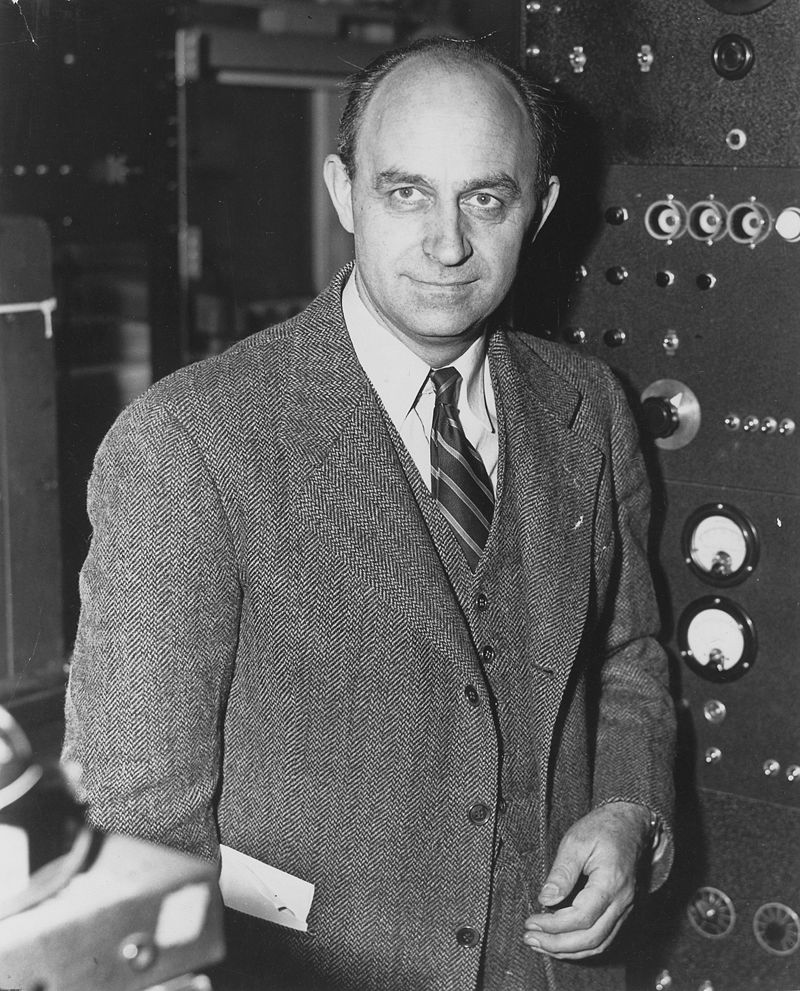
\includegraphics[width=0.8\linewidth]{content/figures/fermi.jpeg}
  \caption{Enrico Fermi (1901–1954)\protect\footnotemark}
\end{figure}


Enrico Fermi (29 September 1901[1] – 28 November 1954) was an Italian physicist, who created the world's first nuclear reactor, the Chicago Pile-1. He has been called the "architect of the nuclear age"[2] and the "architect of the atomic bomb".[3] He was one of the very few physicists in history to excel both theoretically and experimentally. Fermi held several patents related to the use of nuclear power, and was awarded the 1938 Nobel Prize in Physics for his work on induced radioactivity by neutron bombardment and the discovery of transuranic elements. He made significant contributions to the development of quantum theory, nuclear and particle physics, and statistical mechanics.

Fermi's first major contribution was to statistical mechanics. After Wolfgang Pauli announced his exclusion principle in 1925, Fermi followed with a paper in which he applied the principle to an ideal gas, employing a statistical formulation now known as Fermi–Dirac statistics. Today, particles that obey the exclusion principle are called "fermions". Later Pauli postulated the existence of an uncharged invisible particle emitted along with an electron during beta decay, to satisfy the law of conservation of energy. Fermi took up this idea, developing a model that incorporated the postulated particle, which he named the "neutrino". His theory, later referred to as Fermi's interaction and still later as weak interaction, described one of the four fundamental forces of nature. Through experiments inducing radioactivity with recently discovered neutrons, Fermi discovered that slow neutrons were more easily captured than fast ones, and developed the Fermi age equation to describe this. After bombarding thorium and uranium with slow neutrons, he concluded that he had created new elements; although he was awarded the Nobel Prize for this discovery, the new elements were subsequently revealed to be fission products.

Fermi left Italy in 1938 to escape new Italian Racial Laws that affected his Jewish wife Laura Capon. He emigrated to the United States where he worked on the Manhattan Project during World War II. Fermi led the team that designed and built Chicago Pile-1, which went critical on 2 December 1942, demonstrating the first artificial self-sustaining nuclear chain reaction. He was on hand when the X-10 Graphite Reactor at Oak Ridge, Tennessee, went critical in 1943, and when the B Reactor at the Hanford Site did so the next year. At Los Alamos he headed F Division, part of which worked on Edward Teller's thermonuclear "Super" bomb. He was present at the Trinity test on 16 July 1945, where he used his Fermi method to estimate the bomb's yield.

After the war, Fermi served under J. Robert Oppenheimer on the General Advisory Committee, which advised the Atomic Energy Commission on nuclear matters and policy. Following the detonation of the first Soviet fission bomb in August 1949, he strongly opposed the development of a hydrogen bomb on both moral and technical grounds. He was among the scientists who testified on Oppenheimer's behalf at the 1954 hearing that resulted in the denial of the latter's security clearance. Fermi did important work in particle physics, especially related to pions and muons, and he speculated that cosmic rays arose through material being accelerated by magnetic fields in interstellar space. Many awards, concepts, and institutions are named after Fermi, including the Enrico Fermi Award, the Enrico Fermi Institute, the Fermi National Accelerator Laboratory, the Fermi Gamma-ray Space Telescope, the Enrico Fermi Nuclear Generating Station, and the synthetic element fermium, making him one of 16 scientists who have elements named after them.
